% title: Convolutional network (3D feature maps)
% description: VGG-style CNN drawn as pseudo-3D feature-map blocks (thickness = channels, face = spatial size) with conv, pooling, fully connected and softmax stages and shape labels. Add or remove \fmap calls to change the architecture.
\documentclass[tikz,border=10pt]{standalone}
\usepackage{amsmath}
\usetikzlibrary{arrows.meta,calc}

\definecolor{inp}{HTML}{D0D0D0}
\definecolor{conv}{HTML}{F9C784}
\definecolor{pool}{HTML}{E88A8A}
\definecolor{fc}{HTML}{B9A7E0}
\definecolor{soft}{HTML}{9ED6A5}

\tikzset{
  every node/.style={font=\sffamily\scriptsize, align=center},
  flow/.style={-{Stealth[length=1.8mm]}, line width=0.6pt},
}

% \fmap{name}{x}{thickness}{height}{depth}{color}{label}
% x, thickness, height and depth are in millimetres. Defines (name-in) on the left face
% and (name-out) on the right face for arrows.
\newcommand{\fmap}[7]{%
  \pgfmathsetmacro{\ox}{0.45*#5}%
  \pgfmathsetmacro{\oy}{0.35*#5}%
  \pgfmathsetmacro{\xr}{#2+#3}%
  \pgfmathsetmacro{\hh}{#4/2}%
  \filldraw[fill=#6, line width=0.5pt] (#2,-\hh) rectangle (\xr,\hh);
  \filldraw[fill=#6!65!white, line width=0.5pt]
    (#2,\hh) -- ++(\ox,\oy) -- ++(#3,0) -- (\xr,\hh) -- cycle;
  \filldraw[fill=#6!75!black, line width=0.5pt]
    (\xr,-\hh) -- ++(\ox,\oy) -- ++(0,#4) -- (\xr,\hh) -- cycle;
  \coordinate (#1-in) at (#2,0);
  \coordinate (#1-out) at ($(\xr,0)+(0.5*\ox,0.5*\oy)$);
  \node[anchor=north] at ($(#2,-27)+(0.5*#3,0)$) {#7};
}

\begin{document}
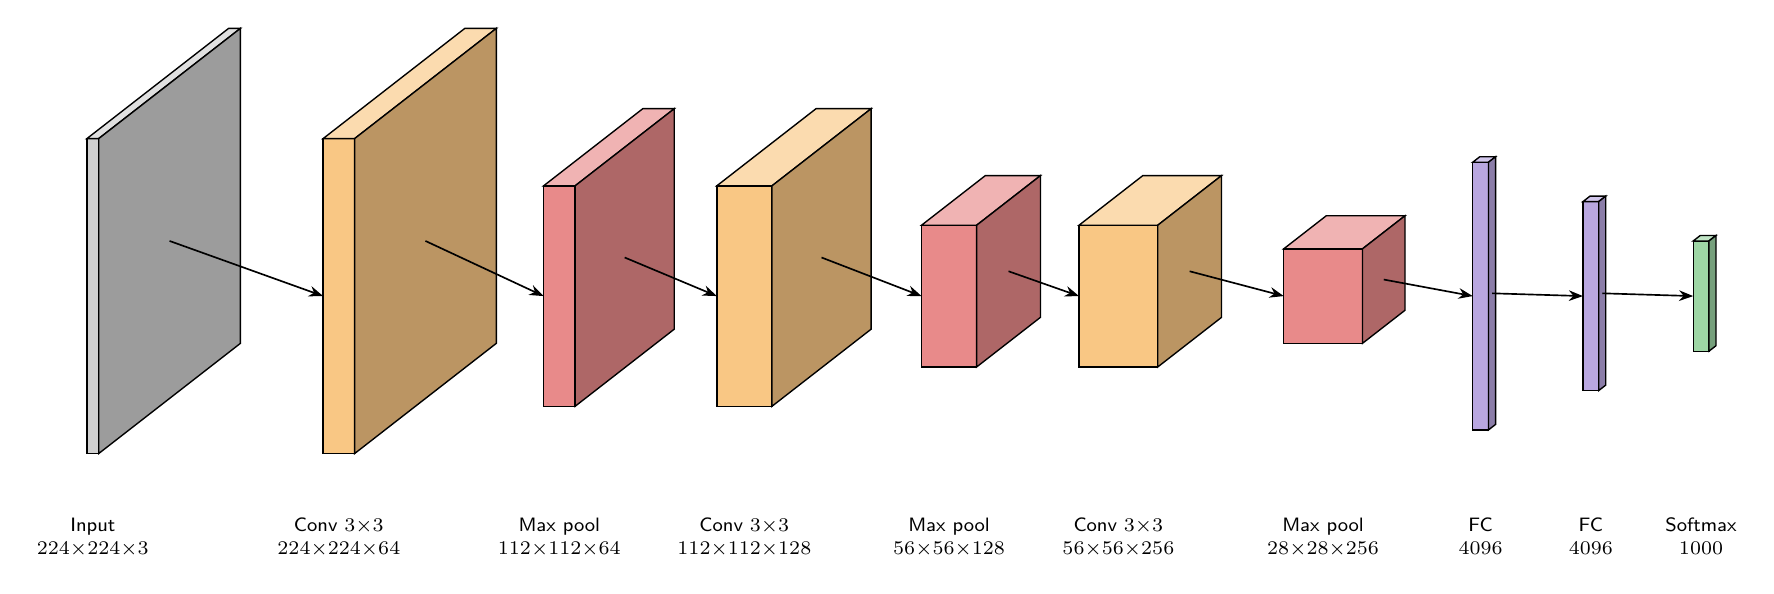
\begin{tikzpicture}[x=1mm, y=1mm]

\fmap{in}{0}{1.5}{40}{40}{inp}{Input\\$224{\times}224{\times}3$}
\fmap{c1}{30}{4}{40}{40}{conv}{Conv $3{\times}3$\\$224{\times}224{\times}64$}
\fmap{p1}{58}{4}{28}{28}{pool}{Max pool\\$112{\times}112{\times}64$}
\fmap{c2}{80}{7}{28}{28}{conv}{Conv $3{\times}3$\\$112{\times}112{\times}128$}
\fmap{p2}{106}{7}{18}{18}{pool}{Max pool\\$56{\times}56{\times}128$}
\fmap{c3}{126}{10}{18}{18}{conv}{Conv $3{\times}3$\\$56{\times}56{\times}256$}
\fmap{p3}{152}{10}{12}{12}{pool}{Max pool\\$28{\times}28{\times}256$}
\fmap{f1}{176}{2}{34}{2}{fc}{FC\\$4096$}
\fmap{f2}{190}{2}{24}{2}{fc}{FC\\$4096$}
\fmap{out}{204}{2}{14}{2}{soft}{Softmax\\$1000$}

\foreach \a/\b in {in/c1, c1/p1, p1/c2, c2/p2, p2/c3, c3/p3, p3/f1, f1/f2, f2/out} {
  \draw[flow] (\a-out) -- (\b-in);
}

\end{tikzpicture}
\end{document}
